\documentclass{article}
\usepackage[left=0.5in,right=0.5in,top=0in,bottom=0in]{geometry}
\usepackage{tikz}
\usetikzlibrary{shapes,arrows,shadows, positioning, calc}
% Define block styles used later

% Interconnection network block
\tikzstyle{intn}=[draw, fill=blue!20, text width=15em, 
    text centered, minimum height=2em]
    
% Directory block
\tikzstyle{d} = [text width=3em, text centered, minimum height=2em,rounded corners,fill=green!20]
% memory block
\tikzstyle{m} = [text width=3em, align=left, minimum height=2em,rounded corners,fill=blue!20]

% Caches
\tikzstyle{ca} = [text width=3em, text centered, minimum height=2em,rounded corners, fill=red!20]

% CPU Blocks

\tikzstyle{cpu} = [text width=3em, text centered, minimum height=2em,fill=yellow!20]
\usepackage{subcaption}

\begin{document}
\begin{figure}
    \centering
    \begin{subfigure}[b]{0.45\textwidth}
            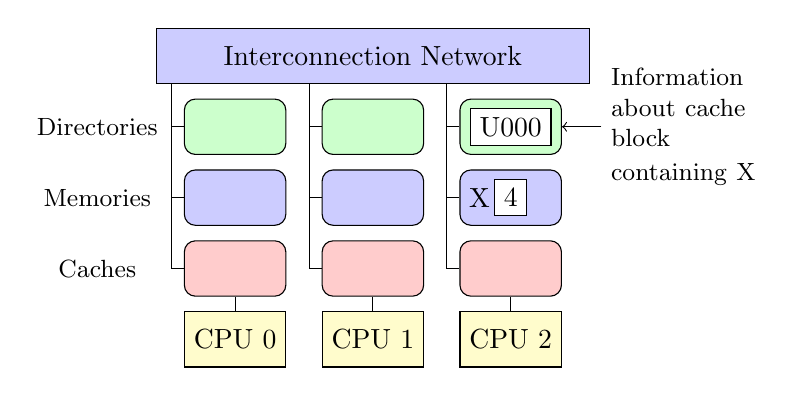
\begin{tikzpicture}[node distance=1.75cm and 1cm] 
            % Block nodes
            \node (in1) [draw, intn] {Interconnection Network};
            \node (d2) [yshift=-0.9cm, draw, d] {};
            \node (d1) [left of = d2, draw, d] {};
            \node (d3) [right of = d2, draw, d] {};
            
            \node (m2) [yshift=-1.8cm, draw, m] {};
            \node (m1) [left of = m2, draw, m] {};
            \node (m3) [right of = m2, draw, m] {X};
            
            
            \node (ca2) [yshift=-2.7cm, draw, ca] {};
            \node (ca1) [left of = ca2, draw, ca] {};
            \node (ca3) [right of = ca2, draw, ca] {};
            
            \node (cpu2) [yshift=-3.6cm, draw, cpu] {CPU 1};
            \node (cpu1) [left of = cpu2,draw, cpu] {CPU 0};
            \node (cpu3) [right of = cpu2, draw, cpu] {CPU 2};
            
            % Node within nodes
            % Label inside node
            \node[draw,fill=white!30] at (d3.center) {U000};
            \node[draw,fill=white!30] at (m3.center) {4};
            % Label nodes, comment out for preceeding diagrams
            \node (dlabel) [left of = d1] {\small{Directories}};
            \node (mlabel) [left of = m1] {\small{Memories}};
            \node (calabel) [left of = ca1] {\small{Caches}};
            
            % Paths to connect all nodes for first column
            \draw ($(in1.south west) +(0.2,0)$) |- (d1.west);
            \draw  (m1.west) -| ($(in1.south west) +(0.2,0) $);
            \draw  (ca1.west) -| ($(in1.south west) +(0.2,0) $);
            
            % Paths for second column
            \draw ($(in1.south west) +(1.95,0)$) |- (d2.west);
            \draw  (m2.west) -| ($(in1.south west) +(1.95,0) $);
            \draw  (ca2.west) -| ($(in1.south west) +(1.95,0) $);
            
            % Paths for third column
            \draw ($(in1.south west) +(3.7,0)$) |- (d3.west);
            \draw  (m3.west) -| ($(in1.south west) +(3.7,0) $);
            \draw  (ca3.west) -| ($(in1.south west) +(3.7,0) $);
            
            % CPU Connections
            \draw (ca1) -- (cpu1);
            \draw (ca2) -- (cpu2);
            \draw (ca3) -- (cpu3);
            
            % arrow outside 
            \node (ulabel) [right = 0.5cm of d3, text width=2cm] {\small{Information about cache block \\ containing X}};
            
            \draw [->] (ulabel) -- (d3.east);
            
            %\draw  (cpu1.west) -| ($(in1.south west) +(0.1,0) $);
            \end{tikzpicture}
            \caption{}
        \end{subfigure}
\hfill %add desired spacing between images, e. g. ~, \quad, \qquad, \hfill etc. 
    %(or a blank line to force the subfigure onto a new line)
\begin{subfigure}[b]{0.45\textwidth}
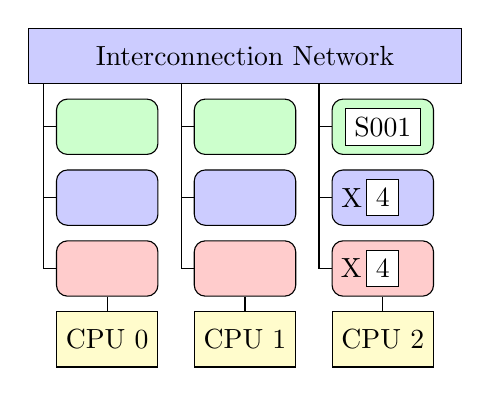
\begin{tikzpicture}[node distance=1.75cm and 1cm] 
% Block nodes
\node (in1) [draw, intn] {Interconnection Network};
\node (d2) [yshift=-0.9cm, draw, d] {};
\node (d1) [left of = d2, draw, d] {};
\node (d3) [right of = d2, draw, d] {};

\node (m2) [yshift=-1.8cm, draw, m] {};
\node (m1) [left of = m2, draw, m] {};
\node (m3) [right of = m2, draw, m] {X};


\node (ca2) [yshift=-2.7cm, draw, ca] {};
\node (ca1) [left of = ca2, draw, ca] {};
\node (ca3) [right of = ca2, draw, ca] {};

\node (cpu2) [yshift=-3.6cm, draw, cpu] {CPU 1};
\node (cpu1) [left of = cpu2,draw, cpu] {CPU 0};
\node (cpu3) [right of = cpu2, draw, cpu] {CPU 2};

% Node within nodes
% Label inside node
\node[draw,fill=white!30] at (d3.center) {S001};
\node[draw,fill=white!30] at (m3.center) {4};

\node[xshift=-0.4cm] at (ca3.center) {X};
\node[draw,fill=white!30] at (ca3.center) {4};
% Label nodes, comment out for preceeding diagrams
% \node (dlabel) [left of = d1] {\small{Directories}};
% \node (mlabel) [left of = m1] {\small{Memories}};
% \node (calabel) [left of = ca1] {\small{Caches}};

% Paths to connect all nodes for first column
\draw ($(in1.south west) +(0.2,0)$) |- (d1.west);
\draw  (m1.west) -| ($(in1.south west) +(0.2,0) $);
\draw  (ca1.west) -| ($(in1.south west) +(0.2,0) $);

% Paths for second column
\draw ($(in1.south west) +(1.95,0)$) |- (d2.west);
\draw  (m2.west) -| ($(in1.south west) +(1.95,0) $);
\draw  (ca2.west) -| ($(in1.south west) +(1.95,0) $);

% Paths for third column
\draw ($(in1.south west) +(3.7,0)$) |- (d3.west);
\draw  (m3.west) -| ($(in1.south west) +(3.7,0) $);
\draw  (ca3.west) -| ($(in1.south west) +(3.7,0) $);

% CPU Connections
\draw (ca1) -- (cpu1);
\draw (ca2) -- (cpu2);
\draw (ca3) -- (cpu3);

%\draw  (cpu1.west) -| ($(in1.south west) +(0.1,0) $);
\end{tikzpicture}
\caption{}
\end{subfigure}
% Row two
\begin{subfigure}[b]{0.3\textwidth}
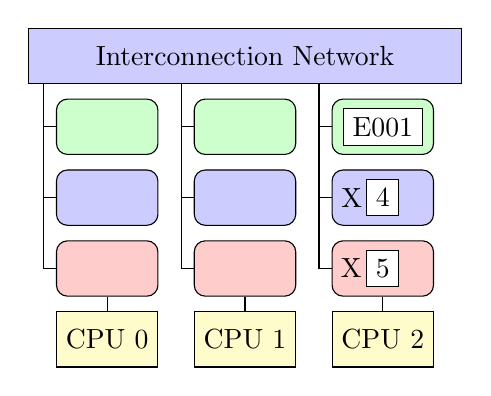
\begin{tikzpicture}[node distance=1.75cm and 1cm] 
% Block nodes
\node (in1) [draw, intn] {Interconnection Network};
\node (d2) [yshift=-0.9cm, draw, d] {};
\node (d1) [left of = d2, draw, d] {};
\node (d3) [right of = d2, draw, d] {};

\node (m2) [yshift=-1.8cm, draw, m] {};
\node (m1) [left of = m2, draw, m] {};
\node (m3) [right of = m2, draw, m] {X};


\node (ca2) [yshift=-2.7cm, draw, ca] {};
\node (ca1) [left of = ca2, draw, ca] {};
\node (ca3) [right of = ca2, draw, ca] {};

\node (cpu2) [yshift=-3.6cm, draw, cpu] {CPU 1};
\node (cpu1) [left of = cpu2,draw, cpu] {CPU 0};
\node (cpu3) [right of = cpu2, draw, cpu] {CPU 2};

% Node within nodes
% Label inside node
\node[draw,fill=white!30] at (d3.center) {E001};
\node[draw,fill=white!30] at (m3.center) {4};

\node[xshift=-0.4cm] at (ca3.center) {X};
\node[draw,fill=white!30] at (ca3.center) {5};
% Label nodes, comment out for preceeding diagrams
% \node (dlabel) [left of = d1] {\small{Directories}};
% \node (mlabel) [left of = m1] {\small{Memories}};
% \node (calabel) [left of = ca1] {\small{Caches}};

% Paths to connect all nodes for first column
\draw ($(in1.south west) +(0.2,0)$) |- (d1.west);
\draw  (m1.west) -| ($(in1.south west) +(0.2,0) $);
\draw  (ca1.west) -| ($(in1.south west) +(0.2,0) $);

% Paths for second column
\draw ($(in1.south west) +(1.95,0)$) |- (d2.west);
\draw  (m2.west) -| ($(in1.south west) +(1.95,0) $);
\draw  (ca2.west) -| ($(in1.south west) +(1.95,0) $);

% Paths for third column
\draw ($(in1.south west) +(3.7,0)$) |- (d3.west);
\draw  (m3.west) -| ($(in1.south west) +(3.7,0) $);
\draw  (ca3.west) -| ($(in1.south west) +(3.7,0) $);

% CPU Connections
\draw (ca1) -- (cpu1);
\draw (ca2) -- (cpu2);
\draw (ca3) -- (cpu3);

%\draw  (cpu1.west) -| ($(in1.south west) +(0.1,0) $);
\end{tikzpicture}
\caption{}
\end{subfigure}
~ %add desired spacing between images, e. g. ~, \quad, \qquad, \hfill etc. 
    %(or a blank line to force the subfigure onto a new line), object d
\begin{subfigure}[b]{0.3\textwidth}
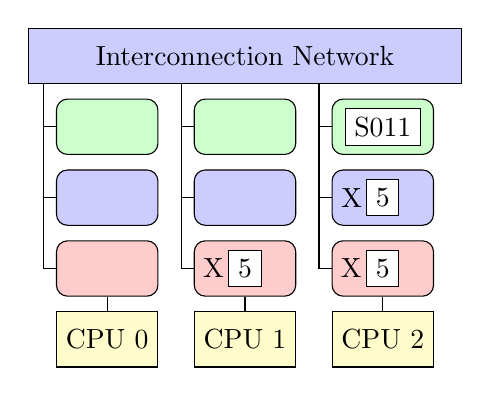
\begin{tikzpicture}[node distance=1.75cm and 1cm] 
% Block nodes
\node (in1) [draw, intn] {Interconnection Network};
\node (d2) [yshift=-0.9cm, draw, d] {};
\node (d1) [left of = d2, draw, d] {};
\node (d3) [right of = d2, draw, d] {};

\node (m2) [yshift=-1.8cm, draw, m] {};
\node (m1) [left of = m2, draw, m] {};
\node (m3) [right of = m2, draw, m] {X};


\node (ca2) [yshift=-2.7cm, draw, ca] {};
\node (ca1) [left of = ca2, draw, ca] {};
\node (ca3) [right of = ca2, draw, ca] {};

\node (cpu2) [yshift=-3.6cm, draw, cpu] {CPU 1};
\node (cpu1) [left of = cpu2,draw, cpu] {CPU 0};
\node (cpu3) [right of = cpu2, draw, cpu] {CPU 2};

% Node within nodes
% Label inside node
\node[draw,fill=white!30] at (d3.center) {S011};
\node[draw,fill=white!30] at (m3.center) {5};

\node[xshift=-0.4cm] at (ca2.center) {X};
\node[draw,fill=white!30] at (ca2.center) {5};

\node[xshift=-0.4cm] at (ca3.center) {X};
\node[draw,fill=white!30] at (ca3.center) {5};
% Label nodes, comment out for preceeding diagrams
% \node (dlabel) [left of = d1] {\small{Directories}};
% \node (mlabel) [left of = m1] {\small{Memories}};
% \node (calabel) [left of = ca1] {\small{Caches}};

% Paths to connect all nodes for first column
\draw ($(in1.south west) +(0.2,0)$) |- (d1.west);
\draw  (m1.west) -| ($(in1.south west) +(0.2,0) $);
\draw  (ca1.west) -| ($(in1.south west) +(0.2,0) $);

% Paths for second column
\draw ($(in1.south west) +(1.95,0)$) |- (d2.west);
\draw  (m2.west) -| ($(in1.south west) +(1.95,0) $);
\draw  (ca2.west) -| ($(in1.south west) +(1.95,0) $);

% Paths for third column
\draw ($(in1.south west) +(3.7,0)$) |- (d3.west);
\draw  (m3.west) -| ($(in1.south west) +(3.7,0) $);
\draw  (ca3.west) -| ($(in1.south west) +(3.7,0) $);

% CPU Connections
\draw (ca1) -- (cpu1);
\draw (ca2) -- (cpu2);
\draw (ca3) -- (cpu3);

%\draw  (cpu1.west) -| ($(in1.south west) +(0.1,0) $);
\end{tikzpicture}
\caption{}
\end{subfigure}
~ 
\begin{subfigure}[b]{0.3\textwidth}
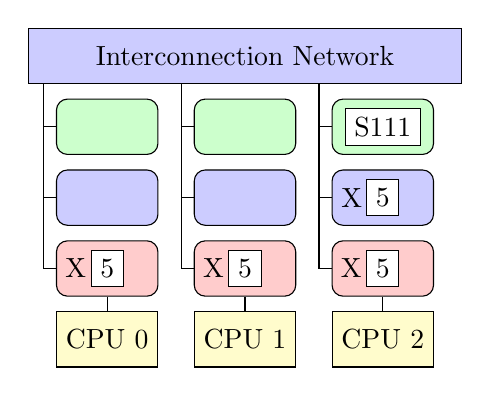
\begin{tikzpicture}[node distance=1.75cm and 1cm] 
% Block nodes
\node (in1) [draw, intn] {Interconnection Network};
\node (d2) [yshift=-0.9cm, draw, d] {};
\node (d1) [left of = d2, draw, d] {};
\node (d3) [right of = d2, draw, d] {};

\node (m2) [yshift=-1.8cm, draw, m] {};
\node (m1) [left of = m2, draw, m] {};
\node (m3) [right of = m2, draw, m] {X};


\node (ca2) [yshift=-2.7cm, draw, ca] {};
\node (ca1) [left of = ca2, draw, ca] {};
\node (ca3) [right of = ca2, draw, ca] {};

\node (cpu2) [yshift=-3.6cm, draw, cpu] {CPU 1};
\node (cpu1) [left of = cpu2,draw, cpu] {CPU 0};
\node (cpu3) [right of = cpu2, draw, cpu] {CPU 2};

% Node within nodes
% Label inside node
\node[draw,fill=white!30] at (d3.center) {S111};
\node[draw,fill=white!30] at (m3.center) {5};

\node[xshift=-0.4cm] at (ca1.center) {X};
\node[draw,fill=white!30] at (ca1.center) {5};

\node[xshift=-0.4cm] at (ca2.center) {X};
\node[draw,fill=white!30] at (ca2.center) {5};

\node[xshift=-0.4cm] at (ca3.center) {X};
\node[draw,fill=white!30] at (ca3.center) {5};
% Label nodes, comment out for preceeding diagrams
% \node (dlabel) [left of = d1] {\small{Directories}};
% \node (mlabel) [left of = m1] {\small{Memories}};
% \node (calabel) [left of = ca1] {\small{Caches}};

% Paths to connect all nodes for first column
\draw ($(in1.south west) +(0.2,0)$) |- (d1.west);
\draw  (m1.west) -| ($(in1.south west) +(0.2,0) $);
\draw  (ca1.west) -| ($(in1.south west) +(0.2,0) $);

% Paths for second column
\draw ($(in1.south west) +(1.95,0)$) |- (d2.west);
\draw  (m2.west) -| ($(in1.south west) +(1.95,0) $);
\draw  (ca2.west) -| ($(in1.south west) +(1.95,0) $);

% Paths for third column
\draw ($(in1.south west) +(3.7,0)$) |- (d3.west);
\draw  (m3.west) -| ($(in1.south west) +(3.7,0) $);
\draw  (ca3.west) -| ($(in1.south west) +(3.7,0) $);

% CPU Connections
\draw (ca1) -- (cpu1);
\draw (ca2) -- (cpu2);
\draw (ca3) -- (cpu3);

%\draw  (cpu1.west) -| ($(in1.south west) +(0.1,0) $);
\end{tikzpicture}
\caption{}
\end{subfigure}
% Row 3
\begin{subfigure}[b]{0.3\textwidth}
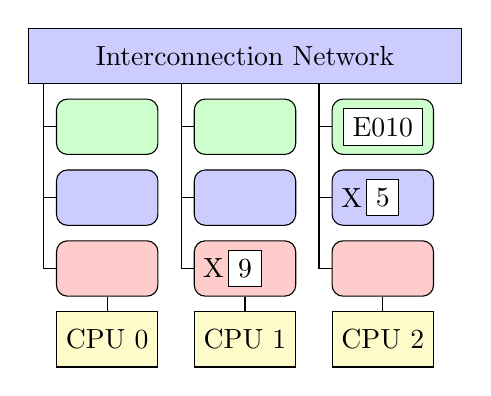
\begin{tikzpicture}[node distance=1.75cm and 1cm] 
% Block nodes
\node (in1) [draw, intn] {Interconnection Network};
\node (d2) [yshift=-0.9cm, draw, d] {};
\node (d1) [left of = d2, draw, d] {};
\node (d3) [right of = d2, draw, d] {};

\node (m2) [yshift=-1.8cm, draw, m] {};
\node (m1) [left of = m2, draw, m] {};
\node (m3) [right of = m2, draw, m] {X};


\node (ca2) [yshift=-2.7cm, draw, ca] {};
\node (ca1) [left of = ca2, draw, ca] {};
\node (ca3) [right of = ca2, draw, ca] {};

\node (cpu2) [yshift=-3.6cm, draw, cpu] {CPU 1};
\node (cpu1) [left of = cpu2,draw, cpu] {CPU 0};
\node (cpu3) [right of = cpu2, draw, cpu] {CPU 2};

% Node within nodes
% Label inside node
\node[draw,fill=white!30] at (d3.center) {E010};
\node[draw,fill=white!30] at (m3.center) {5};

\node[xshift=-0.4cm] at (ca2.center) {X};
\node[draw,fill=white!30] at (ca2.center) {9};

% Label nodes, comment out for preceeding diagrams
% \node (dlabel) [left of = d1] {\small{Directories}};
% \node (mlabel) [left of = m1] {\small{Memories}};
% \node (calabel) [left of = ca1] {\small{Caches}};

% Paths to connect all nodes for first column
\draw ($(in1.south west) +(0.2,0)$) |- (d1.west);
\draw  (m1.west) -| ($(in1.south west) +(0.2,0) $);
\draw  (ca1.west) -| ($(in1.south west) +(0.2,0) $);

% Paths for second column
\draw ($(in1.south west) +(1.95,0)$) |- (d2.west);
\draw  (m2.west) -| ($(in1.south west) +(1.95,0) $);
\draw  (ca2.west) -| ($(in1.south west) +(1.95,0) $);

% Paths for third column
\draw ($(in1.south west) +(3.7,0)$) |- (d3.west);
\draw  (m3.west) -| ($(in1.south west) +(3.7,0) $);
\draw  (ca3.west) -| ($(in1.south west) +(3.7,0) $);

% CPU Connections
\draw (ca1) -- (cpu1);
\draw (ca2) -- (cpu2);
\draw (ca3) -- (cpu3);

%\draw  (cpu1.west) -| ($(in1.south west) +(0.1,0) $);
\end{tikzpicture}
\caption{}
\end{subfigure}
~ 
\begin{subfigure}[b]{0.5\textwidth}
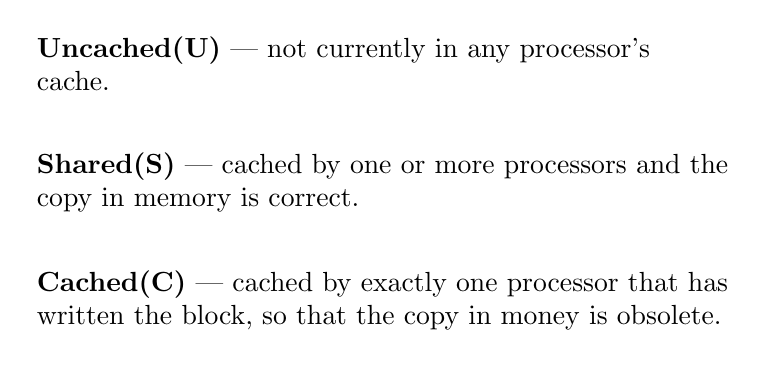
\begin{tikzpicture}[node distance=1.5cm and 1cm] 
\node[text width=25 em] (u){\textbf{Uncached(U)} --- not currently in any processor's cache.};
\node[text width=25 em, below of = u ] (s) {\textbf{Shared(S)} --- cached by one or more processors and the copy in memory is correct.};
\node[text width=25 em, below of = s ] {\textbf{Cached(C)} --- cached by exactly one processor that has written the block, so that the copy in money is obsolete.};
\end{tikzpicture}
\caption{}
\end{subfigure}
%\caption*{Directory-based Cache Operations. (a) Starting Cache from Figure 2.19. (b) State after CPU 2 reads X. (c) State after CPU 2 writes value 5 to X. (d) State after CPU 1 reads X. (e) State after CPU 0 reads X. (f) State after CPU 1 writes value 9 to X.}
\end{figure}
\end{document}